\lstset{style=Python,escapeinside={(*@}{@*)}}


\begin{frame}[fragile]
    Sei $A$ eine $m\times n$-Matrix mit Einträgen
    \begin{align*}
        A =
        \begin{pmatrix}
            a_{1,1} & a_{1,2} & \dots & a_{1,n} \\
            a_{2,1} & a_{2,2} & \dots & a_{2,n} \\
            \vdots  & \vdots  &       & \vdots  \\
            a_{m,1} & a_{m,2} & \dots & a_{m,n} 
        \end{pmatrix}
    \end{align*}
    und $x$ ein Vektor der Länge $n$ mit Einträgen
    \begin{align*}
        x =
        \begin{pmatrix}
            x_1    \\
            x_2    \\
            x_3    \\
            \vdots \\
            x_n
        \end{pmatrix}.
    \end{align*}
\end{frame}

\begin{frame}[fragile]{Matrix-Vektor-Multiplikation}
    \begin{figure}
        \centering
        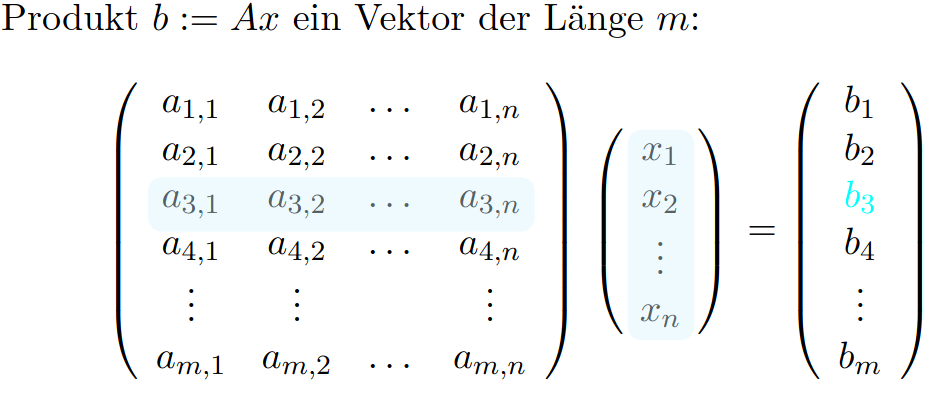
\includegraphics[width=0.9\textwidth]{EF/Complexity/mvm.png}
    \end{figure}
\end{frame}

\begin{frame}[fragile]{Matrix-Vektor-Multiplikation}
    Dabei ist zum Beispiel die Komponente $b_3$ von $b$ gegeben durch die Zahl
    \begin{align*}
        a_{3,1}x_1 + a_{3,2}x_2 + \ldots + a_{3,n}x_n.
    \end{align*}
    Allgemein sind die Komponenten des Matrix-Vektor-Produkts $b=Ax$ gegeben durch
    \begin{align*}
        b_i := \sum_{k=1}^n a_{i,k}x_k = a_{i,1}x_1 + a_{i,2}x_2 + \ldots + a_{i,n}x_n, \quad (i=1,2,\ldots,n). % ** GEÄNDERT (m zu n) **
    \end{align*}
\end{frame}

\begin{frame}[fragile]{Matrix-Vektor-Multiplikation}
    \begin{lstlisting}[escapechar=!, basicstyle=\small]
        // y = Ax
        mvm(A, x, y, n, m)
        {
            for (i = 0; i < m; ++i) !\tikzmark{c1end}!                      !\tikzmark{c1start}!
                for (j = 0; j < n; ++j) !\tikzmark{c2end}!                  !\tikzmark{c2start}!
                    y[i] += A[i*n + j] * x[j]; !\tikzmark{c3end}!           !\tikzmark{c3start}!
        }
    \end{lstlisting}
    \begin{tikzpicture}[overlay, remember picture,
            every node/.style={draw=green!50,fill=green!50!white,text=black,rounded corners}]
        \only<2->{\drawArrow{c1end}{c1start}{\tiny $\text{K:}\; c_1, \text{W:}\; m$}{green!50!white};}
        \only<3->{\drawArrow{c2end}{c2start}{\tiny $\text{K:}\; c_2, \text{W:}\; mn$}{green!50!white};}
        \only<4->{\drawArrow{c3end}{c3start}{\tiny $\text{K:}\; c_3, \text{W:}\; mn$}{green!50!white};}
    \end{tikzpicture}
\end{frame}

\begin{frame}[fragile]{Matrix-Matrix-Multiplikation}
    \begin{figure}
        \centering
        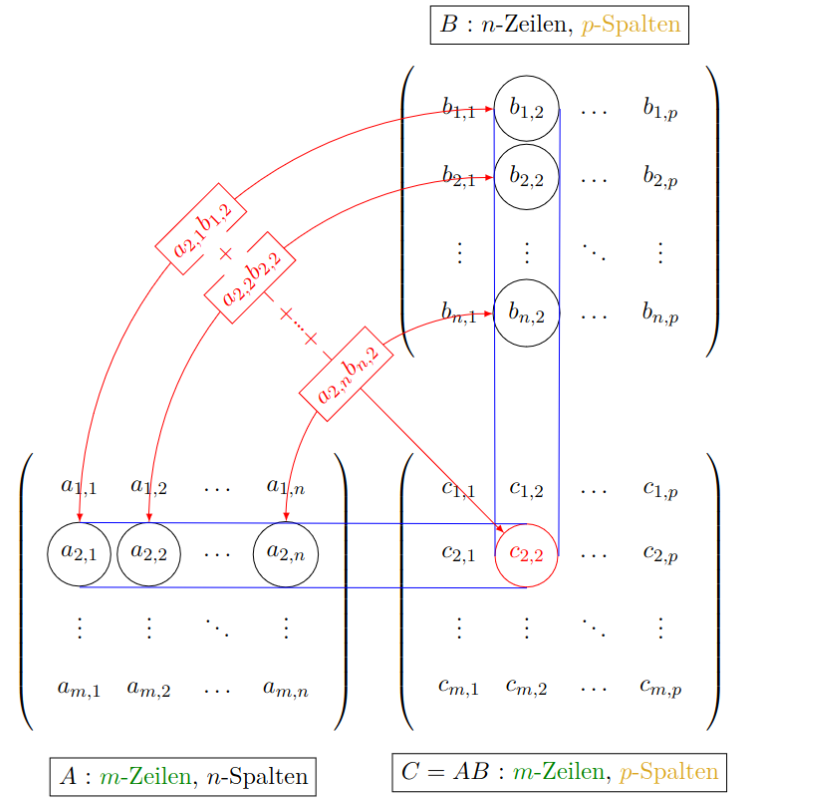
\includegraphics[width=0.7\textwidth]{EF/Complexity/mmm.png}
    \end{figure}
\end{frame}

\begin{frame}
    Im Allgemeinen ist der Eintrag $c_{i,j}$ von $C$ das Vektor-Vektor-Produkt der $i$-ten Zeile von $A$ mit der $j$-ten Spalte von $B$. Deshalb ist es notwendig, dass die \enquote{Breite} von $A$ genau der \enquote{Höhe} von $B$ entspricht. Das Produkt $C=AB$ hat die \enquote{Höhe} von $A$ und die \enquote{Breite} von $B$. Formal definiert man die Einträge von $C$ wie folgt: 
    \begin{align}\label{eq:matrixproduct}
        c_{i,j} := \sum_{k=1}^n a_{i,k}b_{k,j} = a_{i,1}b_{1,j}+a_{i,2}b_{2,j}+\ldots+a_{i,n}b_{n,j},
    \end{align}
    für $(i=1,2,\ldots ,m; j=1,2,\ldots,p)$.
\end{frame}

\begin{frame}[fragile]{Matrix-Matrix-Multiplikation}
    \begin{lstlisting}[escapechar=!, basicstyle=\footnotesize]
        /* Multiply n x n matrices a and b */
        void mmm(double *a, double *b, double *c, int n) {
            int i, j, k; !\tikzmark{c1end}!                                             !\tikzmark{c1start}!
            for (i = 0; i < n; i++) !\tikzmark{c2end}!                                  !\tikzmark{c2start}!
                for (j = 0; j < n; j++) !\tikzmark{c3end}!                              !\tikzmark{c3start}!
                    for (k = 0; k < n; k++) !\tikzmark{c4end}!                          !\tikzmark{c4start}!
                        c[i*n + j] += a[i*n + k]*b[k*n + j]; !\tikzmark{c5end}!         !\tikzmark{c5start}!
        }
    \end{lstlisting}
    \begin{tikzpicture}[overlay, remember picture,
            every node/.style={draw=green!50,fill=green!50!white,text=black,rounded corners}]
        \only<2->{\drawArrow{c1end}{c1start}{\tiny $\text{K:}\; c_1, \text{W:}\; 1$}{green!50!white};}
        \only<3->{\drawArrow{c2end}{c2start}{\tiny $\text{K:}\; c_2, \text{W:}\; n$}{green!50!white};}
        \only<4->{\drawArrow{c3end}{c3start}{\tiny $\text{K:}\; c_3, \text{W:}\; n^2$}{green!50!white};}
        \only<5->{\drawArrow{c4end}{c4start}{\tiny $\text{K:}\; c_4, \text{W:}\; n^3$}{green!50!white};}
        \only<6->{\drawArrow{c5end}{c5start}{\tiny $\text{K:}\; c_5, \text{W:}\; n^3$}{green!50!white};}
    \end{tikzpicture}
\end{frame}

\begin{frame}[fragile]
    \begin{enumerate}
        \item Beschreibe einen Algorithmus, welcher eine Laufzeit von $\Theta\lr{n^4}$ besitzt.
        \item Beschreibe einen Algorithmus, welcher eine Laufzeit von $\Theta\lr{10^n}$ besitzt.
        \item Beschreibe einen Algorithmus, welcher eine Laufzeit von $\Theta\lr{n^{n+1}}$ besitzt.
    \end{enumerate}
\end{frame}

\begin{frame}[fragile]{Best-Case}
    Wie kann fast jeder Algorithmus so modifiziert werden, dass er eine \enquote{schnelle} Best-Case-Laufzeit hat? 
\end{frame}

\begin{frame}{Binary Search}
    \begin{myexercise}[\texttt{binarySearch}]\label{myexercise:binarysearch}
        Implementiere den \texttt{binarySearch} Algorithmus.
    \end{myexercise}
\end{frame}

\begin{frame}{Binary Search}
    \begin{myanswer}
        \lstinputlisting[language=Python,caption=\texttt{binarysearch.py},label=listing:binarysearch, basicstyle=\footnotesize]{Praktikum/Unterrichtsmaterialien/Code/binarysearch.py}
    \end{myanswer}
\end{frame}

\begin{frame}{Analyse von \texttt{binarySearch}}
    \begin{myexercise}[\texttt{binarySearch}]\label{myexercise:binarysearchAnalysis}
        Führen Sie eine Laufzeitanalyse von \texttt{binarySearch} durch. 
    \end{myexercise}
\end{frame}

\begin{frame}[fragile]{Analyse von \texttt{binarySearch}}
    \begin{lstlisting}[escapechar=!, basicstyle=\footnotesize]
            def binary_search(sorted_collection, item): !\tikzmark{c1end}!                      !\tikzmark{c1start}!
                left = 0 !\tikzmark{c2end}!                                                     !\tikzmark{c2start}!
                right = len(sorted_collection) - 1 !\tikzmark{c3end}!                           !\tikzmark{c3start}!

                while left <= right: !\tikzmark{c4end}!                                         !\tikzmark{c4start}!
                    midpoint = left + (right - left) // 2 !\tikzmark{c5end}!                    !\tikzmark{c5start}!
                    current_item = sorted_collection[midpoint] !\tikzmark{c6end}!               !\tikzmark{c6start}!
                    if current_item == item: !\tikzmark{c7end}!                                 !\tikzmark{c7start}!
                        return midpoint !\tikzmark{c8end}!                                      !\tikzmark{c8start}!
                    elif item < current_item:!\tikzmark{c9end}!                                 !\tikzmark{c9start}!
                        right = midpoint - 1!\tikzmark{c10end}!                                 !\tikzmark{c10start}!
                    else: !\tikzmark{c11end}!                                                   !\tikzmark{c11start}!
                        left = midpoint + 1!\tikzmark{c12end}!                                  !\tikzmark{c12start}!
                return -1!\tikzmark{c13end}!                                                    !\tikzmark{c13start}!

    \end{lstlisting}
    \begin{tikzpicture}[overlay, remember picture,
            every node/.style={draw=green!50,fill=green!50!white,text=black,rounded corners}]
        \only<2->{\drawArrow{c1end}{c1start}{\tiny $\text{K:}\; c_1, \text{W:}\; 1$}{green!50!white};}
        \only<3->{\drawArrow{c2end}{c2start}{\tiny $\text{K:}\; c_2, \text{W:}\; 1$}{green!50!white};}
        \only<4->{\drawArrow{c3end}{c3start}{\tiny $\text{K:}\; c_3, \text{W:}\; 1$}{green!50!white};}
        \only<5->{\drawArrow{c4end}{c4start}{\tiny $\text{K:}\; c_4, \text{W:}\; t_i$}{green!50!white};}
        \only<6->{\drawArrow{c5end}{c5start}{\tiny $\text{K:}\; c_5, \text{W:}\; t_i$}{green!50!white};}
        \only<7->{\drawArrow{c6end}{c6start}{\tiny $\text{K:}\; c_6, \text{W:}\; t_i$}{green!50!white};}
        \only<8->{\drawArrow{c7end}{c7start}{\tiny $\text{K:}\; c_7, \text{W:}\; t_i$}{green!50!white};}
        \only<9->{\drawArrow{c8end}{c8start}{\tiny $\text{K:}\; c_8, \text{W:}\; 1$}{green!50!white};}
        \only<10->{\drawArrow{c9end}{c9start}{\tiny $\text{K:}\; c_9, \text{W:}\; t_i$}{green!50!white};}
        \only<11->{\drawArrow{c10end}{c10start}{\tiny $\text{K:}\; c_{10}, \text{W:}\; t_j$}{green!50!white};}
        \only<12->{\drawArrow{c11end}{c11start}{\tiny $\text{K:}\; c_{11}, \text{W:}\; t_i$}{green!50!white};}
        \only<13->{\drawArrow{c12end}{c12start}{\tiny $\text{K:}\; c_{12}, \text{W:}\; t_k$}{green!50!white};}
        \only<14->{\drawArrow{c13end}{c13start}{\tiny $\text{K:}\; c_{13}, \text{W:}\; 1$}{green!50!white};}
    \end{tikzpicture}
    \only<15>{
            Daraus ergibt sich
            \begin{align*}
                c_1 + c_2 + c_3 + c_8 + c_9 + c_{13} + (c_4 + c_5 + c_6 + c_7 + c_9 + c_{11})t_i\\
                 + c_{10} t_j + c_{12} t_k
            \end{align*}
        }
\end{frame}

\begin{frame}[fragile]{Analyse von \texttt{binarySearch}}
    Wie können wir die Terme $t_i$, $t_j$ und $t_k$ näher bestimmen?\pause\\ 
    \begin{itemize}
        \item Im Worst-Case finden wir das Element nicht, oder erst wenn \(left - right \leq 1\). 
        \item In diesem Fall wird in jeder Iteration der While-Schleife entweder Zeile 10 oder Zeile 12 ausgeführt $\rightarrow t_j + t_k = t_i$\pause 
        \item Mit jeder Iteration der While-Schleife verkleinern wir den Suchraum um die Hälfte. 
    \end{itemize}
    \begin{align*}
        &&\frac{n}{2^{t_i}} &\leq 1 &&
        \\\Leftrightarrow && n &\leq 2^{t_i} &&
        \\\Leftrightarrow &&\log_2(n) &\leq t_i && 
    \end{align*}
\end{frame}

\begin{frame}[fragile]{Analyse von \texttt{binarySearch}}
    Daraus ergibt sich
    \begin{align*}
        T(n) & = c_1+c_2+c_3+c_8+c_9 + c_{13} \\
             & + (c_4 + c_5 + c_6 + c_7 + c_9 + c_{11}+\frac{c_{10} + c_{12}}{2})t_i\\
             & \leq c_1+c_2+c_3+c_8+c_9 + c_{13} \\
             & + (c_4 + c_5 + c_6 + c_7 + c_9 + c_{11}+\frac{c_{10} + c_{12}}{2})\log_2(n)\\ 
             & \in O(\log(n)) 
    \end{align*}
\end{frame}

\begin{frame}{Suchen in unbegrenzten Suchräumen}
    Was können wir tun, wenn der Suchraum zwar eine totale Ordnung hat, aber nicht begrenzt ist?\\ 
    Beispiel: Ich überlege mir irgendeine natürliche Zahl. Mit welcher Strategie könntest du vorgehen, um diese Zahl herauszufinden? 
\end{frame}

\begin{frame}{Exponential Search}
    \begin{myexercise}[\texttt{exponentialSearch}]\label{myexercise:exponentialsearch} 
        Implementiere den \texttt{exponentialSearch} Algorithmus. 
    \end{myexercise}
\end{frame}

\begin{frame}{Exponential Search}
    \begin{myanswer}
        \lstinputlisting[language=Python,caption=\texttt{exponentialsearch.py},label=listing:exponentialSearch, basicstyle=\tiny]{Praktikum/Unterrichtsmaterialien/Code/exponentialsearch.py}
    \end{myanswer}
\end{frame}

\begin{frame}{Analyse von \texttt{exponentialSearch}}
    Wie können wir eine Laufzeitanalyse von \texttt{exponentialSearch} durchführen?\pause 
    \begin{myexercise}[\texttt{exponentialSearch}]\label{myexercise:exponentialSearchAnalysis} 
        Führen Sie eine Laufzeitanalyse von \texttt{exponentialSearch} durch. 
    \end{myexercise}
\end{frame}

\begin{frame}{Suchen Lower Bound}
    Bisher haben wir die Laufzeit von Algorithmen analysiert. Als Nächstes wollen wir uns die Frage stellen, ob wir die Komplexität eines Problems bestimmen können.\\ 
    Dies erlaubt es uns, die Qualität eines Algorithmus zu bestimmen. Ein Algorithmus, der das Problem X in der minimalen Zeit löst, ist ein \enquote{guter Algorithmus} für Problem X, unabhängig von seiner eigentlichen Laufzeit. 
\end{frame}

\begin{frame}{Modell}
    Damit wir eine untere Schranke für das Suchen auf sortierten Suchräumen einführen können, brauchen wir ein Modell, das alle vergleichsbasierten Algorithmen abstrahiert. Das heißt, egal wie der Code aussieht, er lässt sich immer in unserem Modell darstellen.\\ 

    \textbf{Beobachtung}: Um einen Wert in einer sortierten Liste zu finden, kann der Computer in jedem Schritt lediglich zwei Werte miteinander vergleichen. Das Ergebnis dieses Vergleichs legt fest, was das Programm im nächsten Schritt tut.\\\pause 

    Wir können dies mit einem Entscheidungsbaum abbilden:
    \begin{itemize}
        \item Jeder Nicht-Blatt-Knoten ist ein Vergleich. 
        \item Jede Kante spezifiziert einen möglichen Ausgang des Vergleichs
        \item Jedes Blatt ist eine mögliche Lösung
    \end{itemize}

    Für jeden Suchalgorithmus können wir den dazugehörigen Entscheidungsbaum bauen. Die Länge des längsten Pfades von der Wurzel zu einem Blatt entspricht der Worst-Case-Laufzeit dieses Suchalgorithmus.
\end{frame}

\begin{frame}{Suchen Lower Bound}
    Um die Komplexität von Suchen auf sortierten Mengen zu begrenzen, zeigen wir, dass jeder Suchbaum eine \textbf{minimale Höhe} haben muss. \\ 
    Das Gesetz der \textbf{Trichotomie} besagt, dass für zwei beliebige Elemente einer total geordneten Menge genau eine der folgenden Beziehungen zutrifft: das erste Element ist kleiner als das zweite, gleich dem zweiten oder größer als das zweite.\\
    Dies bedeutet für unseren Suchbaum, dass jeder Nicht-Blatt-Knoten genau 3 Kinder haben muss. Da es mindestens $n+1$ mögliche Lösungen geben muss ($n$ Positionen oder das Element ist nicht vorhanden), bleibt die Frage, wie hoch ein Baum, in dem jeder Nicht-Blatt-Knoten genau 3 Kinder hat, sein muss, damit er mindestens $n$ Blätter hat. 
\end{frame}

\begin{frame}{Suchen Lower Bound}
    Ein Baum der Höhe $h$, in dem jeder Nicht-Blatt-Knoten drei Kinder hat, hat genau $3^{h}$ Blätter (wobei die Wurzel Höhe 0 hat). Daraus ergibt sich die Ungleichung

    \begin{align*}
        n\leq 3^h\\
        \log_3(n)\leq h
    \end{align*}
    Dies beweist, dass das Suchen auf sortierten Mengen eine minimale Komplexität von $\Omega(\log(n))$ hat.
\end{frame}